\chapter{Teoria rozpoznawania mówcy}\label{chap:teoria}

\section{Przetwarzanie mowy}\label{sec:przetwarzanie_mowy}

\subsection{Mel Frequency Cepstral Coefficients}\label{sec:mfcc}

\shortcut{MFCC}, obok blisko z nimi związanych \foreign{filter banks} stanowią popularny zestaw 
cech dla systemów rozpoznawania mowy i rozpoznawania mówcy. Systemy bazujące na sieciach
neuronowych wykorzystują często nieprzetworzone dalej spektrum sygnału, gdyż obowiązuje
w nich podejście, by zamiast ręcznie przetwarzać wejście lepiej zapewnić sieci neuronowej
architekturę pozwalającą na nauczenie się odpowiednich cech. Na przykład zamiast ręcznie
projektować filtr lepiej dodać do sieci warstwę konwolucyjną. Bardziej tradycyjne metody
oparte o \shortcut{GMM} jednak bardzo korzystają na zredukowaniu wymiarowości problemu
oraz zapewnieniu, że poszczególne cechy są nieskorelowane, co zachodzi przy \shortcut{MFCC}.

Krokiem wstępnym policzenia \shortcut{MFCC} jest \foreign{preemphasis}, czyli przefiltrowanie sygnału 
prostym filtrem wysokoprzepustowym, zwykle postaci $[-0.95, 1.0]$ lub \\ $[-0.97, 1.0]$.

\begin{figure}[H]
    \centering
    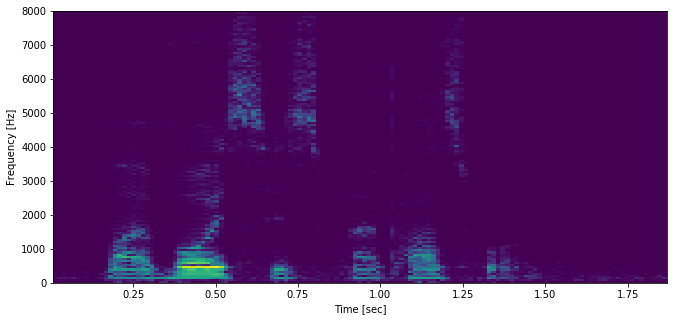
\includegraphics[width=0.8\textwidth]{images/2_1_a_example_spectrogram}
    \caption{Spektrogram sygnału \code{m0002/20150713085938321\underscore m0002\underscore 31.pcm} ze zbioru RedDots}
    \label{fig:2_1_a_example_spectrogram}
\end{figure}

\begin{figure}[H]
    \centering
    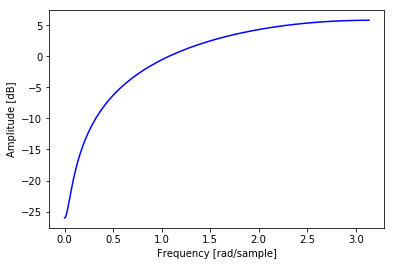
\includegraphics[width=0.6\textwidth]{images/2_1_c_preemphasis_response}
    \caption{Odpowiedź impulsowa \foreign{preemphasis} $[-0.95, 1.0]$}
    \label{fig:2_1_c_preemphasis_response}
\end{figure}

\begin{figure}[H]
    \centering
    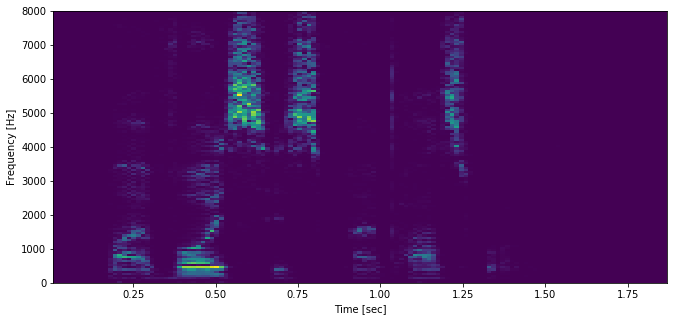
\includegraphics[width=0.8\textwidth]{images/2_1_b_example_preemphasis}
    \caption{Spektrogram tego samego sygnału poddany \foreign{preemphasis}}
    \label{fig:2_1_b_example_preemphasis}
\end{figure}

Jak pokazuje \ref{fig:2_1_b_example_preemphasis}, energia w wyższych pasmach po tej operacji
została wyrównana z energią w niższych pasmach częstotliwości. Ogranicza to błędy numeryczne
pojawiające się przy dalszym przetwarzaniu, co miało duże znaczenie w starszych komputerach.

W drugim kroku należy policzyć \foreign{Short Time Fourier Transform}, to znaczy podzielić
sygnał na ramki i dla każdej ramki policzyć spektrum częstotliwościowe. Typowa szerokość
okna to $25$ms, przy czym każde kolejne okno jest przesunięte o ok. połowę szerokości, 
np. można przyjąć $10$ms. W przypadku zbioru RedDots nagrania mają częstotliwość próbkowania $16$kHz,
więc by uzyskać takie przesunięcie okna muszą zawierać $400$ próbek z przesunięciem $160$ próbek.
Następnie spektra zamieniane są w spektra mocy przez wzięcie kwadratu wartości absolutnej
z każdej wartości w spektrum.

Wynik \shortcut{STFT} można zwizualizować jako spektrogram, jak na \ref{fig:2_1_a_example_spectrogram}, 
i zawiera on informacje o tym jak energia sygnału w różnych pasmach zmieniała się w czasie. 
Każde okno można wyciąć z użyciem okna Hamminga lub Hanna, które mają mniejszy wpływ
na wynikowe spektrum sygnału niż okno prostokątne. (Wycięcie wybranego przedziału próbek
z sygnału jest równoważne przemnożeniu przez okno prostokątne)

Następnie budowany jest bank filtrów w skali Mela. Przeliczenia częstotliwości Melach na
częstotliwość w Hertzach dokonuje się według poniższych wzorów. 

$$m = 2595 log_{10}(1 + \frac{f}{700})$$
$$f = 700 (10^{m/2595} - 1)$$

Jest to skala w nieliniowej zależności z Hertzami. Jej postać i stałe zostały tak dobrane,
że zmiana w tej skali odpowiada subiektywnemu odczuciu zmiany wysokości dźwięku przez ludzi.

Bank filtrów składa się z pewnej liczby, zwykle $20$ lub $26$, trójkątnych filtrów o równej
szerokości w skali Mela, rozmieszczonych z przesunięciem 50\% szerokości. Ich szerokość
jest tak dobrana, by pokryły cały przedział częstotliwości sygnału.

\begin{figure}[H]
    \centering
    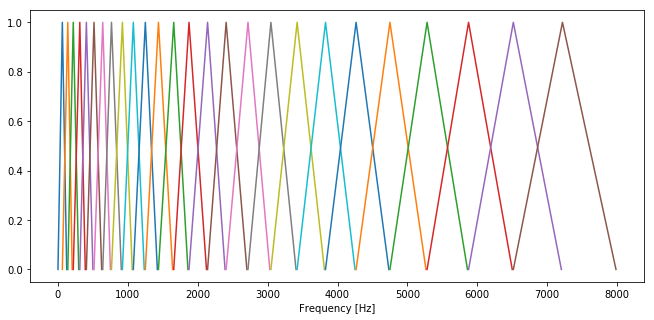
\includegraphics[width=0.8\textwidth]{images/2_1_d_mel_filters}
    \caption{Charakterystyka w skali Hertza banku 20 trójkątnych filtrów o równej szerokości w skali Mela}
    \label{fig:2_1_d_mel_filters}
\end{figure}

Mając te filtry następnym etapem przetwarzania sygnału jest przemnożenie przez każdy z tych filtrów i zsumowanie 
dzięki czemu uzyskuje się jedną liczbę na filtr - całkowitą energię sygnału na pokrytych filtrami pasmach.

Sumy są następnie logarytmowane. Pozwala to na dekonwolucję sygnału mowy i wpływu środowiska. 
Dekonwolucja przebiega w ten sposób, że najpierw dzięki policzeniu transformaty Fouriera,
uzyskiwane jest spektrum, a konwolucja sygnału w czasie jest równoważna przemnożeniu widm częstotliwościowych.
Następnie jak ten iloczyn widm zostanie zlogarytmowany, to oba można go przedstawić jako sumę logarytmów.
W wynikowych cechach jeżeli sygnał mowy został z czymś spleciony, to skutkuje to tylko przesunięciem cech
ze wszystkich ramek. Można wtedy, przy założeniu, że wpływ otoczenia jest stały, znormalizować średnią tych cech, 
by zmniejszyć jego wpływ. 

Znormalizowane współczynniki filtrów Mela bywają używane jako gotowy zestaw cech. Do uzyskania \shortcut{MFCC}
potrzebne jest jeszcze policzenie dyskretnej transformaty cosinusowej. Dyskretna transformata cosinusowa to modyfikacja
transformaty Fouriera, która w wyniku daje ciąg współczynników rzeczywistych, a nie zespolonych. Wykorzystana jest
właściwość \shortcut{DFT}, że jeżeli sygnał w dziedzinie czasu ma współczynniki rzeczywiste, to współczynniki transformaty
będą Hermitian-symetryczne. A jeżeli sygnał w dziedzinie czasu jest symetryczny, to transformata będzie miała
tylko współczynniki rzeczywiste. \shortcut{DCT} liczy się zatem tak, iż tworzony jest nowy sygnał dwa razy większej długości niż
sygnał wyjściowy, przez odbicie wyjściowego sygnału. Taki sygnał będzie symetryczny i rzeczywisty, więc jego transformata
Fouriera będzie również symetryczna i rzeczywista. Połowę transformaty można odrzucić, a druga połowa, zawierająca
współczynniki rzeczywiste i będąca takiego samego rozmiaru co wyjściowy sygnał, nazywamy dyskretną transformatą cosinusową.

Fakt, że \shortcut{DCT} sygnału jest również rzeczywista i ma ten sam rozmiar jest wygodny, lecz liczy się ją, 
gdyż ma właściwości dekorelacyjne. Dzięki temu przy modelowaniu \shortcut{MFCC} za pomocą wielowymiarowej 
dystrybucji normalnej można przyjąć, że
współczynniki są nieskorelowane i zastosować uproszczenie, że macierz kowariancji parametryzująca tę dystrybucję 
jest macierzą diagonalną.

\begin{figure}[H]
    \centering
    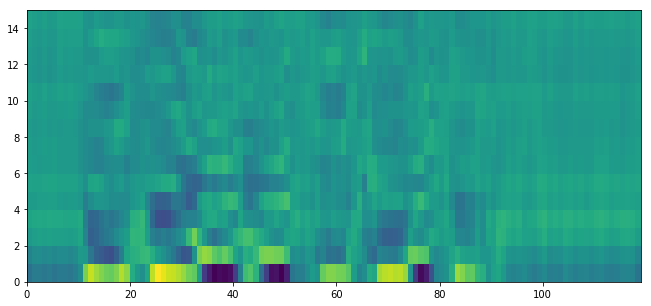
\includegraphics[width=0.8\textwidth]{images/2_1_e_mfcc}
    \caption{Wizualizacja 15 pierwszych współczynników \shortcut{MFCC} dla każdej ramki przykładowego sygnału}
    \label{fig:2_1_e_mfcc}
\end{figure}

Wynik \shortcut{DCT} nazywamy \foreign{Mel-frequency cepstral coefficients} i ze względu na wspomniane właściwości użyjemy ich
w naszych systemach. W praktyce z $26$ współczynników wybiera się tylko pierwsze $13$ lub $20$, gdyż dalsze opisują
wysokie częstotliwości, które są nieprzydatne przy rozumieniu sygnału mowy. Do tych współczynników dołącza się $26$ lub $40$
współczynników delta oraz delta-delta. Współczynniki delta mają opisać jak konkretne współczynniki zmieniają się w czasie,
choć zapewne tracą na przydatności w modelach jak sieci neuronowe, które mogą na wejściu przyjąć nie tylko jedną ramkę sygnału,
ale też kilka sąsiadujących ramek. 

\begin{figure}[H]
    \centering
    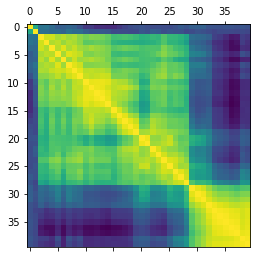
\includegraphics[width=0.6\textwidth]{images/2_1_f_correlation_matrix_banks}
    \caption{Macierz korelacji dla współczynników uzyskanych z banku filtrów}
    \label{fig:2_1_f_correlation_matrix_banks}
\end{figure}

\begin{figure}[H]
    \centering
    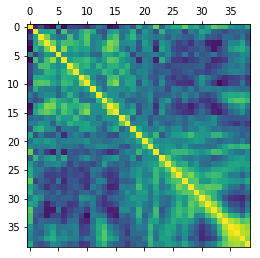
\includegraphics[width=0.6\textwidth]{images/2_1_g_correlation_matrix_mfcc}
    \caption{Macierz korelacji dla współczynników \shortcut{MFCC}}
    \label{fig:2_1_g_correlation_matrix_mfcc}
\end{figure}

\subsection{Mikstury gaussowskie}\label{sec:gmm}

Mikstura rozkładów to sposób opisu rozkładu zmiennej losowej $X$ przez wprowadzenie dodatkowej ukrytej zmiennej $\Theta$.
Następnie uznaje się, że dla każdej wartości zmiennej ukrytej rozkład zmiennej pochodzi z innego rozkładu.
Zwykle zmienna ukryta jest dyskretna, wyjściowa zmienna może być dyskretna lub ciągła i przyjmuje się, że wszystkie
warunkowe rozkłady $P(X|\Theta)$ pochodzą z tej samej rodziny i różnią się parametrami. Rozkład zmiennej $X$ można
uzyskać przez marginalizację zmiennej ukrytej.

$$f(x) = \sum_{\theta_i} f(X | \theta_i) P(\theta_i)$$

Przy miksturach gaussowskie przyjmuje się, że warunkowe prawdopodobieństwa zmiennej wyjściowej od zmiennej ukrytej
należą do rodziny wielowymiarowych rozkładów normalnych, tj. mają gęstość

$$f(x | \theta_i) = \frac{1}{\sqrt{(2 \pi)^d |\Sigma_i|}} exp(-\frac{1}{2} (x - \mu_i)^T \Sigma_i^{-1} (x - \mu_i))$$

gdzie $\mu_i$ to $d$ wymiarowy wektor średnich, $\Sigma_i$ to macierz kowariancji rozmiaru $d \times d$

\subsection{Maksymalizowanie wartości oczekiwanej}\label{sec:gmm}

Parametry wielowymiarowego rozkładu normalnego można wyestymować na podstawie próby, na przykład 
stosując estymator maksymalizujący prawdopodobieństwo danych.

Estymatory parametrów maksymalizujące prawdopodobieństwo $M$ elementów $x^j$.

$\hat{\mu} = \frac{1}{m} \Sigma_{j=0}^M x^{j}$

$\hat{\Sigma} = \frac{1}{m} \Sigma_{j=0}^M (x^{j} - \hat{\mu})^T (x^{j} - \hat{\mu})$

Jednak w przypadku mikstury, jeżeli nie przypiszemy z góry próbek wybranym wartościom ukrytej zmiennej, problem 
estymacji parametrów wymaga innego podejścia. Jedną z metod jest \foreign{Expectation Maximization}, iteracyjny 
algorytm wyznaczania wartości parametrów dla mikstur dystrybucji lub ogólniej dla modeli z ukrytymi zmiennymi. 
Składa się z dwóch kroków wykonywanych na zmianę do zbieżności:

\begin{itemize}
    \item \foreign{Expectation} -  % todo
    \item \foreign{Maximization} - 
\end{itemize}

Algorytm nie gwarantuje znalezienia globalnie optymalnego rozwiązania.

\subsection{Dynamic Time Warping}\label{sec:dtw}

Jako że praca dotyczy rozpoznawania zależnego od tekstu, konieczne by uzyskać wartościowe wyniki będzie
użycie metod pozwalających na uwzględnienie informacji o sekwencji ramek. Samo dopasowanie mikstur do ramek
tej informacji nie uwzględni. Jedną z takich metod jest \foreign{dynamic time warping}.

\shortcut{DTW} to algorytm do porównywania dwóch ciągów. Ciągi mogą być różnej długości i algorytm zwróci
dla nich wysokie podobieństwo (małą odległość) nawet jeśli pewne podciągi będą bardziej rozciągnięte lub krótsze 
w jednym ciągu niż w drugim. 

Algorytm wymaga wybrania metryki (oznaczmy ją $d$) określającą odległość pojedynczych elementów ciągu.

\shortcut{DTW} wykorzystuje technikę programowania dynamicznego i w podstawowej wersji znanej autorowi wymaga liczby operacji 
rzędu $\Theta(n \times m)$, gdzie $n$ i $m$ to długości porównywanych ciągów oraz ma złożoność pamięciową liniową
względem długości krótszego ciągu. Istnieją jego bardziej wydaje wersje, w tym wersje z oknem, tzn. bazujące na 
założeniu, że nie ma sensu porównywać elementów z dwóch ciągów ze zbyt odległymi indeksami.

Algorytm wygląda tak: Na początku inicjalizowana jest macierz odległości $D$ rozmiaru $n + 1 \times m + 1$. Pierwszy
rząd i pierwsza kolumna jest wypełniana cyfrową reprezentacją $\infty$, co oznacza tyle, 
że te wartości nie są brane pod uwagę w następnym kroku.
Wyjątkiem jest komórka w pierwszym rzędzie i pierwszej kolumnie z wartością $D_{0,0} = 0$.

Pozostałe wartości macierzy są liczone ze wzoru

$$D_{i+1, j+1} = min(D_{i+1, j}, D_{i, j+1}, D_{i, j}) + d(N_i, M_j)$$

gdzie $N_i$ i$M_j$ oznaczają elementy porównywanych ciągów, a $d(N_i, M_j)$ to jak już wspomniano wybrana 
niezależnie od algorytmu odległość między dwoma elementami. Odległość ciągów od siebie znaleziona przez \shortcut{DTW}
to $D_{n, m}$.  Licząc te wartości rzędami możliwe jest osiągnięcie liniowej złożoności pamięciowej względem
długości krótszego ciągu.

Powyższy wzór na $D_{i+1, j+1}$ należy zinterpretować tak, że liczymy odległość pary elementów $N_i$, $M_j$ i dodajemy
do najbardziej korzystnego wyniku z pośród trzech opcji:

\begin{itemize}
    \item Wybór $D_{i+1, j}$ oznacza, że obecny rezultat składa się z $d(N_i, M_{j-1})$ i $d(N_i, M_j)$, a więc ten sam element ciągu $N$ jest porównany z dwoma elementami ciągu $M$. Na przykład w $N = [1, 20, 20, 20, 20]$, $M = [1, 1, 1, 10]$ i odległości różnicy absolutnej ten przypadek będzie kilka razy najkorzystniejszy.
    \item Wybór $D_{i, j+1}$ oznacza, że w sumie będzie zarazem $d(N_{i-1}, M_j)$ i $d(N_i, M_j)$, a więc dwa elementy ciągu $N$ są porównane z tym samym elementem ciągu $M$. Na przykład w wyniku dla $N = [1, 1, 1, 1, 1, 20]$ i $ M = [1, 10]$ ten przypadek będzie się składał na wynik minimalizujący odległość ciągów.
    \item $D_{i, j}$ oznacza, że obliczono odległość następnego elementu zarówno z ciągu $N$ i z ciągu $M$. Przy porównywaniu $N = [1, 2, 3, 4]$ oraz $M = [1, 2, 3, 4]$ zajdzie wyłącznie on.
\end{itemize}

Poniżej przedstawiono kilka przykładów tabelek z wynikami $DTW$. Elementami są liczby, a w roli metryki jest kwadrat różnicy.

\begin{table}[H]
    \caption{Macierz $D$ dla $DTW$ na dwóch przykładowych sekwencjach $N$ i $M$. Przykład gdy elementy jednej sekwencja są wielokrotnie dopasowana do pierwszego elementu z drugiej sekwencji, dopóki jest to możliwe.}
    \centering
    \label{tab:dtw_example0}
    \small
    \tabulinesep =_3pt^3pt
    \begin{tabu}{r*{7}{r}}
        \multirow{2}{*}{} & & \multicolumn{5}{c}{N}
        \\
        & & - & 1 & 20 & 20 & 20 & 20
        \\ \midrule
        \multirow{5}{*}{M} & - & 0 & $\infty$ & $\infty$ & $\infty$ & $\infty$ & $\infty$
        \\ 
        & 1 & $\infty$ & 0 & 19 & 38 & 57 & 76
        \\
        & 1 & $\infty$ & 0 & 19 & 38 & 57 & 76
        \\
        & 1 & $\infty$ & 0 & 19 & 38 & 57 & 76
        \\
        & 10 & $\infty$ & 9 & 10 & 20 & 30 & \textbf{40}
        \\
    \end{tabu}
\end{table}

\begin{table}[H]
    \caption{Macierz $D$ dla $DTW$ na dwóch przykładowych sekwencjach $N$ i $M$. Przykład z dokładnie dopasowanymi sekwencjami, z wydłużonymi lub skróconymi fragmentami.}
    \centering
    \label{tab:dtw_example1}
    \small
    \tabulinesep =_3pt^3pt
    \begin{tabu}{r*{11}{r}}
        \multirow{2}{*}{} & & \multicolumn{9}{c}{N}
        \\
        & & - & 1 & 1 & 2 & 3 & 3 & 3 & 4 & 4
        \\ \midrule
        \multirow{7}{*}{M} & - & 0 & $\infty$ & $\infty$ & $\infty$ & $\infty$ & $\infty$ & $\infty$ & $\infty$ & $\infty$
        \\
        & 1 & $\infty$ & 0 & 0 & 1 & 3 & 5 & 7 & 10 & 13
        \\
        & 2 & $\infty$ & 1 & 1 & 0 & 1 & 2 & 3 & 5 & 7
        \\
        & 2 & $\infty$ & 2 & 2 & 0 & 1 & 2 & 3 & 5 & 7
        \\
        & 2 & $\infty$ & 3 & 3 & 0 & 1 & 2 & 3 & 5 & 7
        \\
        & 3 & $\infty$ & 5 & 5 & 1 & 0 & 0 & 0 & 1 & 2
        \\
        & 4 & $\infty$ & 8 & 8 & 3 & 1 & 1 & 1 & 0 & \textbf{0}
        \\
    \end{tabu}
\end{table}

\subsection{Ukryte modele Markowa}\label{sec:hmm}

Ukryty model Markowa to proces stochastyczny, dyskretny w czasie, pozwalający na modelowanie dystrybucji 
sekwencji zdarzeń. Będzie zatem użyteczny ze względu na możliwość uwzględnienia w nim zależności 
między ramkami w czasie.

Model składa się z zbioru $N$ ukrytych stanów $X = \{x_0, x_1, \dots\, x_{N-1}\}$, ciągu zmiennych losowych
$X_t$, $t = 0, 1, \dots, T - 1$ oznaczających ukryty stan w chwili $t$, rozkładu początkowego stanu ukrytego
$\pi_i = P(X_0 = x_i)$, zbioru obserwacji (emisji, stan jawny) $Y$, przy czym obserwacje mogą być dyskretne 
lub ciągłe i ciągu zmiennych losowych $Y_t$, $t = 0, 1, \dots, T - 1$ określających obserwację w chwili $t$.

Do tego zdefiniowane są prawdopodobieństwa przejść między stanami oraz rozkłady obserwacji w każdym stanie. 
Kluczową kwestią w modelu Markowa, zwaną regułą Markowa, jest iż rozkład prawdopodobieństwo następnego stanu $X_t$ 
zależy wyłącznie od stanu poprzedzającego, nie jest ważna cała historia stanów w przeszłości. Podobnie rozkład
obserwacji $Y_t$ zależy wyłącznie od obecnego stanu ukrytego. 

Inną właściwością, którą się przyjmuje, jest jednorodność. Oznacza to, że przejścia między stanami i emisje są
niezależne od czasu $t$. Przy dyskretnych i jednorodnych stanach ukrytych prawdopodobieństwa przejść
między stanami można zapisać w postaci macierzy $H$ (\foreign{transition matrix}) $P(X_t = x_i | X_{t-1} = x_j) = H_{j, i}$.
Podobnie jeżeli emisje są dyskretne, to można je zapisać w postaci macierzy $V$ $P(Y_t = y_i | X_t = x_j) = V_{j, i}$.
Lecz emisje często mają jakieś określone parametryczne dystrybucje i wtedy definiuje się w postaci wektorów parametrów.
$H$ (oraz $V$ jeżeli mowa o dyskretnych emisjach) jest macierzą stochastyczną, więc $\forall_{i, j = 0 \dots N - 1} 0 \leq H_{i, j} \leq 1$ i $\forall_{i = 0 \dots N - 1} \sum_{j = 0}^{N - 1} H_{j, i} = 1$. (rzędy sumują się do 1)

Czasami, w innych modelach regułę Markowa rozszerza się tak, iż prawdopodobieństwo może zależeć od $k$ ostatnich stanów
$P(X_t | X_{t-1} \dots X_{t-k})$ i nazywa się to regułą Markowa $k$ rzędu. Są też inne wersje, w których zbiór
ukrytych stanów jest ciągły, w których rząd $k$ jest zmienny lub na przykład pola Markowa, 
gdzie nie mówimy o ciągu w czasie, lecz o zmiennych rozmieszczonych
w kilku wymiarach, których wartości zależą od pewnego sąsiedztwa. Wszystkie modele Markowa mają jednak cechę wspólną, iż
zmienne losowe zależą w nich od pewnego skończonej liczby innych zmiennych.

Jeżeli macierz przejść jest tak zdefiniowana, że zawsze możliwe jest przejście z każdego stanu do każdego, to
mówimy, że model jest ergodyczny. Jednak na przykład w rozpoznawaniu mowy często definiuje się macierz przejść,
by pozwalała tylko na przejście do stanu o takim samym lub wyższym indeksie, tzw. model Bakisa lub model lewo-prawo 
(\foreign{left-to-right}) albo by miała niezerowe prawdopodobieństwo przejścia wyłącznie z danego stanu do jego 
samego lub stanu o indeksie o jeden większym. (model \foreign{beads-on-string})

Ważne w praktyce jest, że istnieją wydajne algorytmy rozwiązujące następujące problemy \shortcut{HMM}.

\begin{enumerate}
    \item Algorytm w przód - problem znalezienia prawdopodobieństwa stanu ukrytego w danej chwili wraz z pewnym ciągiem obserwacji do tego chwili. Jeżeli tym punktem w czasie będzie koniec sekwencji obserwacji, to można zmarginalizować prawdopodobieństwo końcowego stanu i uzyskać prawdopodobieństwo wygenerowania danej sekwencji obserwacji przez model.
    \item Algorytm w tył - problem znalezienia prawdopodobieństwa ciągu zdarzeń w przyszłości, pod warunkiem danego stanu ukrytego w danej chwili. Jest on istotny, gdyż jest częścią następnego algorytmu.
    \item Algorytm w przód i w tył - problem znalezienia prawdopodobieństwa stanu ukrytego w danej chwili pod warunkiem wystąpienia danego ciągu obserwacji. Brany pod uwagę jest cały ciąg obserwacji, tych przed i tych po danym stanie ukrytym. Działa przez połączenie wyników algorytmu w przód i w tył, stąd nazwa. 
    \item Algorytm Viterbiego - problem znalezienia najbardziej prawdopodobnego ciągu stanów ukrytych dla danego ciągu obserwacji parametrów modelu. Jest podobny do algorytmu w przód, z tym, że na każdym kroku wybiera najbardziej prawdopodobną sekwencję zamiast uwzględniać prawdopodobieństwa wszystkich stanów.
    \item Algorytm Bauma-Welcha - problem znalezienia parametrów modelu Markowa (prawdopodobieństwo przejść między stanami ukrytymi, rozkład obserwacji dla każdego stanu ukrytego, rozkład stanu początkowego) maksymalizującego prawdopodobieństwo wystąpienia danego ciągu obserwacji. Wykorzystuje algorytm w przód i w tył oraz opisany wcześniej algorytm \foreign{expectation maximization}, algorytm \foreign{forward-backward} służy do wyznaczenia ukrytych zmiennych opisujących jaki był stan w każdej chwili czasu na potrzeby kroku \foreign{expectation}, a następnie wyznaczane są najbardziej prawdopodobne parametry emisji w kroku \foreign{maximization}.
\end{enumerate}

Poniżej wyprowadzono te algorytmy, zakładając przy tym dyskretne emisje.

\subsubsection{Algorytm w przód}

Algorytm w przód (\foreign{Forward algorithm}) liczy łączone prawdopodobieństwo znalezienia się w jakimś stanie w chwili $t$
i wystąpienia pewnego ciągu obserwacji $y_{t-1} \dots y_0$ w przeszłości. 

To znaczy liczy $P(x_t, y_t \dots y_0)$. Korzysta z rekurencyjnej zależności

$$P(x_t, y_t \dots y_0) = \sum_{x_{t-1}} P(x_t, x_{t-1}, y_t \dots y_0) =$$
$$\sum_{x_{t-1}} P(y_t | x_t, x_{t-1}, y_{t-1} \dots y_0) P(x_t | x_{t-1}, y_{t-1} \dots y_0) P(x_{t-1}, y_{t-1} \dots y_0)$$

Dzięki własności Markowa można to uprościć do:

$$P(y_t | x_t, x_{t-1}, y_{t-1} \dots y_0) = P(y_t | x_t) = V_{x_t, y_t}$$  

$$P(x_t | x_{t-1}, y_{t-1} \dots y_0) = P(x_t | x_{t-1}) = H_{x_{t-1}, x_t}$$

Ostateczną zależnością jest

$$P(x_t, y_t \dots y_0) = V_{x_t, y_t} \sum_{x_{t-1}} H_{x_{t-1}, x_t} P(x_{t-1}, y_{t-1} \dots y_0) $$

gdzie $P(x_{t-1}, y_{t-1} \dots y_0)$ może być rekurencyjnie obliczone w ten san sposób aż do przypadku bazowego $P(x_0, \emptyset) = \pi_1$, gdzie $\pi$ to rozkład początkowy.

Użycie własności Markowa pozwala zredukować złożoność obliczeniową problemu z $\theta(MN^M)$ do $\theta(MN^2)$, gdzie $M$ to możliwa liczba obserwacji, a $N$ to liczba stanów ukrytych.

\subsubsection{Algorytm w tył}

Algorytm w tył (\foreign{backward algorithm}), jest podobny do algorytmu w przód. Oblicza $P(y_{t+1} \dots y_{T-1} | x_t)$, to znaczy prawdopodobieństwo wystąpienia wskazanej sekwencji obserwacji $y_{t+1} \dots y_{T-1}$, gdzie $T$ to liczba obserwacji, zakładając początkowy stan ukryty $x_t$ w chwili $t$. Obliczenia zaczyna się od końcowego stanu $x_{T-1}$.

$$P(y_{t+1} \dots y_{T-1} | x_t) = \sum_{x_{t+1}} P(y_{t+1} \dots y_{T-1}, x_{t+1} | x_t) =$$
$$\sum_{x_{t+1}} P(y_{t+1} | y_{t+2} \dots y_{T-1}, x_{t+1}, x_t) P(y_{t+2} \dots y_{T-1} | x_{t+1}, x_t) P(x_{t+1} | x_t)$$

Now we can hopefully simplify:

$$P(y_{t+1} | y_{t+2} \dots y_{T-1}, x_{t+1}, x_t) = P(y_{t+1} | x_{t+1}) = V_{x_{t+1},y_{t+1}}$$

$$P(y_{t+2} \dots y_{T-1} | x_{t+1}, x_t) = P(y_{t+2} \dots y_{T-1} | x_{t+1})$$

$$P(x_{t+1} | x_t) = H_{x_t,x_{t+1}}$$

Ostateczna zależność to:

$$P(y_{t+1} \dots y_{T-1} | x_t) =  \sum_{x_{t+1}} V_{x_{t+1},y_{t+1}} H_{x_t,x_{t+1}} P(y_{t+2} \dots y_{T-1} | x_{t+1})$$

Prawdopodobieństwo jest liczone rekurencyjnie, aż do przypadku bazowego $P(\emptyset | x_{T-1}) = 1$

\subsubsection{Algorytm w przód i w tył}
Algorytm w przód i w tył (\foreign{Forward-Backward algorithm}) działa przez połączenie wyników algorytmu w przód i w tył.

Przypomnijmy, że:

\begin{enumerate}
    \item Algorytm w przód oblicza $P(x_t, y_t \dots y_0)$, to znaczy prawdopodobieństwo dla ukrytego stanu w chwili $t$ oraz ciągu stanów z przeszłości.
    \item Algorytm w tył oblicza $P(y_{T-1} \dots y_{t+1} | x_t)$, czyli warunkowe prawdopodobieństwo ciągu obserwacji z przyszłości wobec ukrytego stanu w chwili $t$.
    \item Algorytm w przód i w tył oblicza $P(x_t | y_{T-1} \dots y_0)$. Oblicza zatem prawdopodobieństwo ukrytego stanu $x_t$ w dowolnej chwili $t$ biorąc pod uwagę całą ciąg obserwacji. Możliwe jest dzięki niemu wybranie najbardziej prawdopodobnego stanu w każdej chwili. Trzeba zauważyć, że biorąc najbardziej prawdopodobny stan z każdej chwili niekoniecznie uzyska się najbardziej prawdopodobny ciąg stanów ukrytych odpowiadający ciągowi obserwacji, bo przejście z jednego bardzo prawdopodobnego stanu do drugiego może być bardzo nieprawdopodobne. Dlatego do tego zadania służy algorytm Viterbiego.
\end{enumerate}

Wynik \foreign{Forward-Backward} wykorzystuje poprzednie dwa algorytmy tak:

$$P(x_t, y_t \dots y_0) P(y_{T-1} \dots y_{t+1} | x_t) = P(y_t \dots y_0 | x_t) P(y_{T-1} \dots y_{t+1} | x_t) P(x_t) = $$
$$P(y_{T-1} \dots y_0 | x_t) P(x_t) = P(y_{T-1} \dots y_0, x_t) = P(x_t | y_{T-1} \dots y_0) P(y_{T-1} \dots y_0)$$

$$P(x_t | y_{T-1} \dots y_0) = \frac{P(x_t, y_t \dots y_0) P(y_{T-1} \dots y_{t+1} | x_t)}{P(y_{T-1} \dots y_0)}$$

Prawdopodobieństwo w mianowniku można wyznaczyć przez zsumowanie po $X_{T-1}$ w wynikach algorytmu w przód $\sum_{x_{T-1}} P(x_{T-1}, y_{T-1} \dots y_0)$

\subsubsection{Algorytm Bauma-Welcha}

Algorytm Bauma-Welcha (\foreign{Baum-Welch algorithm}) pozwala na znalezienie najbardziej prawdopodobnych parametrów
$H$, $\pi$, $V$ (lub innych zależnie od emisji) modelu Markowa zależnie od ciągu obserwacji. Algorytm bazuje na metodzie
\foreign{expectation-maximization}. Wykorzystuje przy tym algorytm w przód i w tył (\foreign{forward-backward}) 
do znalezienia w kroku \foreign{expectation} prawdopodobieństw ukrytych stanów dla danej sekwencji obserwacji. 
W kroku \foreign{maximization} estymuje parametry szukając takich, które maksymalizują prawdopodobieństwo wystąpienia
obserwacji, przy założeniu takich ukrytych stanów jak to wyznaczono w poprzednim kroku. Operacje te są powtarzane.

Jak próbowano pokazać powyżej algorytm \foreign{forward-backward} pozwala obliczyć $P(x_t | y_{T-1} \dots y_0)$, 
łącząc $P(x_t, y_t \dots y_0)$ $P(y_{T-1} \dots y_{t+1} | x_t)$ liczone przez algorytmy \foreign{forward} i \foreign{backward}.

Do przeprowadzenia treningu \foreign{Bauma-Welcha} potrzebne jest dodatkowo wyznaczenie $P(x_t, x_{t+1} | y_{T-1} dots y_0)$, 
czyli prawdopodobieństwa przejścia z jednego stanu w chwili $t$ do drugiego w chwili $t+1$, 
uwzględniając sekwencję $T$ obserwacji i, niejawnie, parametrów modelu. 

$$P(x_t, x_{t+1} | y_{T-1} dots y_0)
= \frac{P(x_t, x_{t+1}, y_{T-1} dots y_0)}{P(y_{T-1} dots y_0)}$$

$$P(x_t, x_{t+1}, y_{T-1} dots y_0) = P(y_{T-1} dots y_0 | x_t, x_{t+1}) P(x_{t+1} | x_t) P(x_t) = $$
$$P(y_{T-1} \dots y_{t+2} | x_t, x_{t+1}) P(y_{t+1} \dots y_0 | x_t, x_{t+1}) P(x_{t+1} | x_t) P(x_t)$$

$$P(y_{t+1} \dots y_0 | x_t, x_{t+1}) P(x_t) = P(y_{t+1} \dots y_0, x_t | x_{t+1}) = $$
$$P(y_{t+1} | x_{t+1}) P(y_t \dots y_0, x_t | x_{t+1})$$

$$P(x_t, x_{t+1}, y_{T-1} \dots y_0) =$$
$$P(y_{T-1} \dots y_{t+2} | x_t, x_{t+1}) P(y_{t+1} | x_{t+1}) P(y_t \dots y_0, x_t | x_{t+1}) P(x_{t+1} | x_t) =$$
$$P(y_{T-1} \dots y_{t+2} | x_{t+1}) P(y_{t+1} | x_{t+1}) P(y_t \dots y_0, x_t) P(x_{t+1} | x_t)$$

$$P(x_t, x_{t+1} | y_{T-1} \dots y_0)
= \frac{P(y_{T-1} \dots y_{t+2} | x_{t+1}) P(y_t \dots y_0, x_t) V_{x_{t+1}, y_{t+1}} H_{x_t, x_{t+1}}}{P(y_{T-1} \dots y_0)}$$

Wtedy można uaktualniać parametry w ten sposób, zakładając dyskretne obserwacje opisane macierzą stochastyczną. Inaczej trzeba użyć odpowiedniego estymatora.

$$\pi_i = P(X_0 = x_i | y_{T-1} \dots y_0)$$

$$H_{x_t, x_{t+1}} = \frac{\sum_{t=0}^{T-1} P(x_t, x_{t+1} | y_{T-1} \dots y_0)}{\sum_{t=0}^{T-1} P(x_t | y_{T-1} \dots y_0)}$$

$$V_{x_t, y_t} = \frac{\sum_{t=0}^{T-1} \mathbb{1}_{Y_t = y_t} P(x_t | y_{T-1} \dots y_0)}{\sum_{t=1}^T P(x_t | y_{T-1} \dots y_0)}$$

\subsubsection{Algorytm Viterbiego}

Używając algorytmu \foreign{forward-backward} można obliczyć prawdopodobieństwa dla każdego stanu w każdej chwili, biorąc
pod uwagę cały ciąg obserwacji $P(x_t | y_{T-1} \dots y_0)$. Można by wziąć najbardziej prawdopodobny stan z każdej chwili,
lecz nie dałoby to koniecznie najbardziej prawdopodobnej sekwencji stanów ukrytych, gdyż możliwa jest sytuacja, że
prawdopodobieństwo przejścia między dwoma wybranymi stanami byłoby bardzo małe lub niemożliwe i w efekcie wystąpienie 
i jednego i drugiego z nich w jednym ciągu byłoby mało prawdopodobne.

Algorytm Viterbiego (\foreign{Viterbi algorithm}) rozwiązuje problem znalezienia najbardziej prawdopodobnej sekwencji ukrytych stanów pod warunkiem danego ciągu obserwacji, $x_{T-1} \dots x_0$ maksymalizującego $P(x_{T-1} \dots x_0 | y_{T-1} \dots y_0)$. 

Algorytm wykorzystuje technikę programowania dynamicznego. Tworzy dwie matrycę, oznaczmy je $A$ i $B$.

$$A_{t,x_i} = max_{x_1 \dots x_{t-1}} P(x_1 \dots x_{t-1}, X_t = x_i, y_0 \dots y_t)$$ 
czyli zawiera największe prawdopodobieństwo jakie może mieć ciąg stanów $x_0 \dots x_{t-1}$ wraz z zajściem ciągu obserwacji $y_0 \dots y_t$ oraz z prawdopodobieństwem, że w następnym kroku stanem będzie $x_i$ .

$$B_{t,x_i} = argmax_{x_1 \dots x_{t-1}} P(x_1 \dots x_{t-1}, X_t = x_i, y_0 \dots y_t)$$ i służy do odtworzenia na koniec, które ukryte stany wchodzą w skład wybranej ścieżki. Warto zauważyć, że w tym przypadku $t > 0$.

Mając $A_{t,x_i}$, algorytm oblicza prawdopodobieństwo dla następnej chwili czasu $A_{t+1,x_i}$ w taki sposób:

$$P(x_1 \dots x_t, y_0 \dots y_t) = P(y_t | x_1 \dots x_t, y_0 \dots y_{t-1}) P(x_1 \dots x_t, y_0 \dots y_{t-1}) =$$
$$P(y_t | x_1 \dots x_t, y_0 \dots y_{t-1}) P(x_t | x_1 \dots x_{t-1}, y_0 \dots y_{t-1}) P(x_1 \dots x_{t-1}, y_0 \dots y_{t-1}) =$$
$$P(y_t | x_t) P(x_t | x_{t-1}) P(x_1 \dots x_{t-1}, y_0 \dots y_{t-1}) =$$
$$V_{x_t, y_t} H_{x_{t-1}, x_t} P(x_1 \dots x_{t-1}, y_0 \dots y_{t-1})$$

$$A_{t,x_i} = max_{x_1 \dots x_{t-1}} P(x_1 \dots x_{t-1}, X_t = x_i, y_0 \dots y_t) =$$
$$max_{x_1 \dots x_{t-1}} V_{x_i, y_t} H_{x_{t-1}, x_i} P(x_1 \dots x_{t-1}, y_0 \dots y_{t-1}) =$$
$$V_{x_i, y_t} max_{x_{t-1}}(H_{x_{t-1}, x_i} A_{t-1, x_{t-1}})$$

Przypadek bazowy to $A_{1,x_i} = P(X_1 = x_i, y_0) = \pi_i V_{x_i, y_0}$

Jeśli chodzi o $B$, to zachowuje argumenty, dla których w $A$ jest maksimum:

$$B_{t, x_i} = argmax_{x_1 \dots x_{t-1}} P(x_1 \dots x_{t-1}, X_t = x_i, y_0 \dots y_t) =$$
$$argmax_{x_{t-1}} H_{x_{t-1}, x_i} A_{t-1, x_{t-1}}$$

Po zakończeniu obliczeń możemy znaleźć najbardziej prawdopodobną ścieżkę stanów przez wybranie stanu $x_i$ z największym prawdopodobieństwem w chwili $T-1$ i odtworzyć całą ścieżkę korzystając z $B$.

% cite Rabiner Tutorial

\section{Rozpoznawanie mówcy}\label{sec:rozpoznawanie_mowcy}

W naszej pracy nad systemami rozpoznawania mówcy wyróżniliśmy trzy etapy działania: treningu (\foreign{train}), 
zapisów (\foreign{enrollment}) i prób (\foreign{trial}). Jest to podział inspirowany podziałem w zbiorze RedDots.

W czasie treningu model jest uczony na możliwie dużym zbiorze danych i przez być może długi czas. W czasie zapisów
jest on dostosowywany do wybranego mówcy na podstawie możliwie małego zbioru nagrań wyłącznie tego mówcy. Jest
to istotne, gdyż proces nagrywania może być uciążliwy i ze względów praktycznych byłoby lepiej, gdyby wymagał
jak najmniej pracy ze strony rejestrowanej osoby. W czasie prób następuje weryfikacja mówcy na podstawie niewidzianych
wcześniej nagrań.

\subsection{MAP adaptacja}

MAP adaptation of speaker-independent model to a speaker of parameters is obtained by solving 

$$\frac{d}{d\lambda} P(\lambda | O) = 0$$

where

$$P(\lambda | O) = \frac{P(O | \lambda)P(\lambda)}{P(O)}$$

If we have a good prior estimated from a lot of data, then we can use it to get a model for a speaker for which data is scarce.

Conjugate priors for a random vector is defined as the prior distribution for the parameters of the parameters of the probaiblity density function of the random vector, such that the posterior distribution $P(\lambda | O)$ and the prior distribution $P(\lambda)$ belong to the same distribution family for any sample observations $O$.
For example, it is well known that the conjugate prior for the mean of a Gaussian density is also a Gaussian density.

$$\bar{u_{MAP}} = \frac{n \tau^2}{\sigma^2 + n \tau^2} \bar{o} + \frac{\sigma^2}{\sigma^2 + n \tau^2} \rho$$

where $\bar{o}$ - sample mean of new data, $n$ - number of training observations, $\tau^2$ - variance of prior, $\rho$ - mean of prior distribution

How do we estimate $\rho$ and $\tau^2$ of prior? From a collection of speaker-dependent models (and $c_m$ is a weight of a model) or from a speaker-independent model with mixture of distributions in each state ($c_m$ is a weight of a mixture component)

$\rho = \sum_{m=1}^M c_m \rho_m$

$\tau^2 = \sum_{m=1}^M c_m (\rho_m - \rho)$

% cite Rabiner book

\subsection{i-wektory}
%C Utterance Verification for Text-Dependent Speaker Recognition: aComparative Assessment Using the RedDots Corpus

I-wektory polegają na reprezentowaniu nagrań w postaci S = m + Tw, gdzie w to i-wektor, S to nagranie, m to UBM-superwektor, T to macierz niskiego rzędu

\subsection{PLDA}

% \subsection{JFA}

\subsection{Krzywa ROC}

\foreign{Receiver operating characteristic}

\foreign{Equal error rate}

\foreign{Area under curve}

\subsection{LSTM}

\section{Istniejące systemy weryfikacji mówcy}\label{sec:istniejace_systemy}

%%% Text-independent
\subsection{Metody niezależne od tekstu}

%%% GMM UBM   
Jednym ze sposobów weryfikacji mówcy stosowanym od dawna jest \shortcut{GMM-UBM}. Polega on na utworzeniu modelu tła
(\foreign{universal background model}), modelu mikstur gaussowskich i dopasowaniu ich do ramek \shortcut{MFCC} z nagrań
treningowych. Następnie, do każdego mówcy tworzony jest osobny model przez \shortcut{MAP} adaptację modelu tła do nagrań danego
mówcy. W 
%C Utterance Verification for Text-Dependent Speaker Recognition: aComparative Assessment Using the RedDots Corpus
następnie dokonywane liczona jest różnica między logarytmem prawdopodobieństwa wygenerowania nagrania przez model
dla mówcy i przez model tła. Różnica ta porównywana jest z progiem i na tej podstawie podejmowana jest decyzja
o weryfikacji. Podobnie można weryfikować treść nagrania, przez adaptację modelu tła do nagrań konkretnej treści.
Jeżeli treść wszystkich wypowiedzi jest znana i jest to zbiór zamknięty, to zamiast porównywać model dla jednej 
treści z modelem tła, radzą wykorzystać \foreign{mean norm} lub \foreign{max norm}. To znaczy porównać wynik weryfikowanego
modelu ze średnim wynikiem pozostałych lub z najlepszym wynikiem pozostałych. Autorzy mają podejście, by niezależnie
zweryfikować mówcę i treść wypowiedzi.

Autorzy testują wiele modeli, w tym zarówno do weryfikacji mówcy i treści mają \shortcut{GMM-UBM} z 512 miksturami. 
Jako cechy używają 19 \shortcut{MFCC} z delta i delta-delta cechami. \shortcut{MAP}-adaptacja z \foreign{relevance factor} 3. 
Do weryfikacji mówcy przy adaptacji korzystają z nagrań tego mówcy, a do weryfikacji treści nagrań tej samej treści.

%%% GMM i-vectors PLDA
Podejście z miksturami można rozwinąć. Bardzo popularnym rozwinięciem są i-wektory, w których zamiast liczyć log-prawdopodobieństwo liczone są wektory charakteryzujące mówcę, a następnie do odpowiedzenia na problem weryfikacji wykorzystywane 
jest \shortcut{LDA}, które jest metodą nadzorowanego klastrowania.

Na przykład w
%C Utterance Verification for Text-Dependent Speaker Recognition: aComparative Assessment Using the RedDots Corpus
zastosowano i-wektory do weryfikacji mówcy. Trenują \shortcut{GMM-UBM} z 512 miksturami, osobno dla każdej płci.
I-wektor ma rozmiar 400, i-wektor dla danego mówcy jest średnią z wszystkich i-wektorów dla jego nagrań. 
Długość i-wektorów jest następnie normalizowana. Do weryfikacji użyte jest 
\foreign{gaussian probabilistic linear discriminant analysis}. (\shortcut{g-PLDA})

%%% GMM i-vectors JFA

\subsection{Metody zależne od tekstu}

%%% Text-dependent
%C Parallel Speaker and Content Modelling for Text-dependent Speaker Verification
Powyższe systemy nie uwzględniają kolejności w jakiej ramki powinny być w wypowiedzi. W problemie weryfikacji
zależnej od tekstu jest to jednak możliwe i powinno pozwolić na poprawienie skuteczności systemu.
W \shortcut{GMM-UBM} te same mikstury uczestniczą niezależnie od czasu, a i-wektory są uśredniane dla całej
wypowiedzi. Na szczęście dzięki użyciu \shortcut{HMM} lub \shortcut{DTW} możliwe jest uwzględnienie tych informacji.

%%% DTW

%%% HMM GMM (i-vectors PLDA / JFA)

W pracy
%C Parallel Speaker and Content Modelling for Text-dependent Speaker Verification
pracy utworzono kilka modeli \shortcut{HMM} z emisjami \shortcut{GMM}. Autorzy osobno 
zajmują się problemem weryfikacji mówcy i weryfikacji treści. Używany jest zbiór RedDots.

Najpierw tworzą \shortcut{HMM} dla każdej frazy w ten sposób, że emisje modelu są inicjalizowane przez 
skopiowanie parametrów \shortcut{UBM}, 
a następnie dotrenowane z użyciem wszystkich nagrań treningowych z pewnym zdaniem. 
Następnie dla każdego mówcy model danego zdania jest kopiowany i MAP-adaptowany do jego nagrań tego zdania. 
Przy weryfikacji mówcy za pomocą algorytmu Viterbiego obliczany jest logarytm 
prawdopodobieństwa, że nagranie pochodzi od danego mówcy oraz że nagranie pochodzi od \shortcut{HMM} tła. 
Ocena nagrania to różnica między tymi wynikami i system decyduje o weryfikacji porównując ten wynik z pewnym progiem.

Następnie tworzą drugi podsystem do weryfikacji treści. Dzielą nagrania tej samej frazy na pewną liczbę segmentów
i tworzą dla każdej frazy \shortcut{HMM} typu \foreign{left-to-right}. Jako, że nagrań jest mało, to trudno
wytrenować model, by był w stanie wykryć, które ramki zawierają jakie fony, dlatego segmenty dzielą na sztywno
i właściwie ręcznie dopasowują mikstury do ramek. Weryfikacja frazy przebiega w ten sposób, że liczą średnią
różnicę w log-prawdopodobieństwie między pochodzeniem frazy z odpowiedniej dla mówcy i segmentu mikstury, a
pochodzeniem ramki z \shortcut{GMM UBM}. (nie \shortcut{HMM})

Użyli 19 \shortcut{MFCC} z delta i delta-delta cechami. \shortcut{GMM-UBM} ma 512 mikstur. \shortcut{MAP} adaptacja 
dotyczy tylko wektora średnich. Liczba segmentów w drugiej części to 4 i 8, lecz 8 nie poprawiło im wyników. Liczba 
stanów HMM w pierwszej części to 4 lub 8 i 8 lekko poprawiło im wyniki.

Podobny pomysł jest wykorzystany w jednym z systemów do weryfikacji treści w 
%C Utterance Verification for Text-Dependent Speaker Recognition: aComparative Assessment Using the RedDots Corpus
Wytrenowali 512 miksturowy \shortcut{GMM UBM}. Ich HMM jest typu \foreign{left-to-right} z 5 stanami. 
Naukę rozpoczynając dzieląc jedno nagranie na 5 równych segmentów. 
Każdy z 5 \shortcut{GMM} emitujących \shortcut{MAP}-adaptują z modelu tła korzystając z próbek odpowiedniego segmentu.
Pozostałe nagrania są dzielone na segmenty korzystając z tego modelu. Następnie trenują ostateczne modele dla każdej
wypowiedzi \shortcut{MAP}-adaptując model tła korzystając z wszystkich nagrań, zakładając podział na ramki jak
w poprzednim kroku.

W 
%c COMPARISON OF MULTIPLE FEATURES AND MODELING METHODS FORTEXT-DEPENDENT SPEAKER VERIFICATION
model \shortcut{HMM} został bardziej rozwinięty. Wykorzystano wiedzę o treści wypowiedzi w postaci transkrypcji,
Mając transkrypcje można lepiej dopasować \shortcut{GMM}, niż używając jednego zestawu bardzo wielu mikstur 
do każdej ramki ten sam zestaw.
Można wykorzystać model stworzony na potrzeby rozpoznawania mowy.
Taki model ma stany ukryte, które mają odpowiadać fonemom języka. Na przykład angielski ma 39 fonemów, czemu odpowiadałoby 39 stanów, lecz powszechne jest rozszerzenie
modelu do 3 stanów na jeden fonem, co ma pozwolić osobno określić cechy dla początka, środka i końca fonemu. 
Bardziej złożone systemy, jak HTK
% cite HTK book
, dodatkowo pozwalają na zbudowanie tzw. modelu trójfonowego (\foreign{triphone}), co oznacza, że nie używają trzech stanów na fonem, lecz
przypisują inne stany w zależności od fonemu bezpośrednio przed i bezpośrednio po danym fonemie. Powoduje to duży wzrost wymaganych stanów, to znaczy z $3 \times 39$ do $3 \times 39^3$,
dlatego te systemy dodatkowo łączą bardzo podobne trójki, by dzieliły ze sobą mikstury. Określenie podobieństwo bazuje na wiedzy o podziałach głosek i tym jak układ głosowy przechodzi między nimi.
W 
% cite COMPARISON OF MULTIPLE FEATURES AND MODELING METHODS FORTEXT-DEPENDENT SPEAKER VERIFICATION
użyto modelu jednofonowego (\foreign{monophone}), choć użyli też trójfonowego w nieco innym przypadku. 

Do modelowania emisji używa się GMM. Jako, że stanów jest dużo więcej niż w \shortcut{GMM-UBM} lub w \shortcut{HMM}, w którym wypowiedź jest podzielona na 4-5 części, to
w opisanym przykładzie tego modelu zastosowane jest 8 mikstur zamiast 512 lub 1024. Wyjątkiem są ramki, gdzie spodziewana jest cisza (początek, koniec i przerwa między wyrazami), tam
użyto 16 mikstur. Warto zauważyć, że we front-endzie użyto 20 \shortcut{MFCC} wziętych z banku filtrów rozmiaru 40 i dołączono cechy delta i delta-delta.

Mając taki model można użyć algorytmu Viterbiego lub \foreign{forward-backward}, by przypisać ramkom z nagrania fonemy, które na nich występują. Dla każdego mówcy
przez \shortcut{MAP}-adaptację można stworzyć ich własny zestaw mikstur do każdego stanu i potem weryfikować mówcę przez porównanie logarytmu prawdopodobieństwa
pochodzenia nagrania od mówcy, a pochodzenia od modelu do rozpoznawania mowy, tak jak w opisanej wcześniej \shortcut{GMM-UBM}. 

Zamiast tego na przykład w tej pracy
% cite i-vector/HMM Based Text-dependent Speaker Verification Systemfor RedDots Challenge
użyto \shortcut{HMM}, lecz dokonując rejestracji i weryfikacji z wykorzystaniem metody i-wektorów. W przeciwieństwie do poprzedniej pracy, tu \shortcut{HMM} jest jednofonowy. Autorzy przetestowali
i-wektory rozmiaru 400 oraz 600 i dokonują weryfikacji przez obliczenie podobieństwa cosinusowego.

\subsection{Metody wykorzystujące sieci neuronowe}

%%% HMM with DNN-based senone posteriors (TDNN)

%%% Bottleneck features d-vectors


Choć \foreign{bottleneck features} dają dobre rezultaty w weryfikacji niezależnej od tekstu, to w weryfikacji zależnej
sprawdzają się gorzej niż \shortcut{MFCC}.
%c COMPARISON OF MULTIPLE FEATURES AND MODELING METHODS FORTEXT-DEPENDENT SPEAKER VERIFICATION

%%% Googlowe end-to-end LSTM g-vectors

